%\RequirePackage{fix-cm}
\documentclass[12pt,a4paper]{article}
% Load Package
% \usepackage{blindtext} % optional filler-text package; not required for build
\usepackage{graphicx}
\usepackage{multicol}
\usepackage{tabularx}
\usepackage{booktabs}
\usepackage{pgffor}
\usepackage{color}
\usepackage[hyperfootnotes=true,colorlinks=true,allcolors={blue}]{hyperref}
\usepackage{indentfirst}
\usepackage{dcolumn}
\usepackage{nameref}
% \usepackage{placeins} % optional; missing in current TeX install
\usepackage{flafter}  % put this in your pre-amble
\usepackage{float} % to manage figure float
% \usepackage{authblk} % not used; missing in current TeX install
% \usepackage{dirtytalk} % not used; missing in current TeX install
\usepackage{siunitx} % for the \nombre command
%\usepackage{cite}
\usepackage{bookmark}
%\usepackage{lmodern}
%\usepackage{mathptmx} % for nice font
%\fontfamily{cmss}
\usepackage{mathtools}
\usepackage{exscale}
% \hypersetup{
%   colorlinks=true,
%   allcolors=blue
% }

% \usepackage{threeparttable} % not used; missing in current TeX install
\usepackage{booktabs, longtable}
\usepackage{tabularx}
\usepackage[singlelinecheck=false]{caption}
% for source under image
\usepackage{caption}
%\newcommand{\source}[1]{\fontsize{7}{8}\selectfont Source: {#1}}
\newcommand{\source}[1]{\caption*{\fontsize{7}{8}\selectfont Source: {#1}} }

% for accessibility 
\newcommand{\alt}[1]{\caption*{\fontsize{9}{11}\selectfont Alt text: {#1}} }


% page setup
\usepackage{geometry} % for margin
\geometry{
  left=20mm,
  right=20mm,
  top=20mm,
  bottom=20mm,
  heightrounded,% better use it
}
\usepackage{setspace}
\onehalfspacing

\usepackage{url}
\usepackage[
	backend=biber,
	style=authoryear,
	sorting=ydnt,
	citestyle=authoryear,
	natbib=true
]{biblatex}
\addbibresource{citations.bib}


\makeatletter
\newcommand{\myfnsymbol}[1]{%
  \expandafter\@myfnsymbol\csname c@#1\endcsname
}
% Mapping of how the symbols will be interpreted sequentially
\newcommand{\@myfnsymbol}[1]{%
  \ifcase #1
    % 0
  \or 1% 1
  \or 2% 2
  \or 3% 3
  \or \TextOrMath{\textasteriskcentered}{*}% 4
  \or \TextOrMath{\textdagger}{\dagger}% 5
  \fi
}

\newcommand{\affiliationA}{\@myfnsymbol{1}}
\newcommand{\affiliationB}{\@myfnsymbol{2}}
\makeatother



\makeatletter
\newcommand{\myfnsymbol}[1]{%
  \expandafter\@myfnsymbol\csname c@#1\endcsname
}
% Mapping of how the symbols will be interpreted sequentially
\newcommand{\@myfnsymbol}[1]{%
  \ifcase #1
    % 0
  \or 1% 1
  \or 2% 2
  \or 3% 3
  \or \TextOrMath{\textasteriskcentered}{*}% 4
  \or \TextOrMath{\textdagger}{\dagger}% 5
  \fi
}

\newcommand{\affiliationA}{\@myfnsymbol{1}}
\newcommand{\affiliationB}{\@myfnsymbol{2}}

\makeatother

\title{\textbf{Estimating the Influence of Demographic Ageing and Migration to the Spanish Aggregate Labour Supply}}

\author{
  Gilbert Montcho\textsuperscript{\affiliationA}\\
  Alejandro Steven Fonseca-Zendejas\textsuperscript{\affiliationB}\\
  Marcel Mérrete\textsuperscript{\affiliationA}
}

\begin{document}


\renewcommand{\thefootnote}{\myfnsymbol{footnote}}
\maketitle

% Layout the notes in order
\footnotetext[1]{Department of Economics, University of Ottawa, Ottawa, Quebec, Canada}%
\footnotetext[2]{Department of Economics, Universidad Loyola Andalucía, Seville, Spain}%

\setcounter{footnote}{0}% Restart footnote counter
% Footnotes for rest of document uses \fnsymbol 
\renewcommand{\thefootnote}{\fnsymbol{footnote}}

% show abstract on the title page
\begin{abstract}

Population ageing has raised concerns about the future of aggregate labour supply, but its effects depend not only on the rising share of older individuals, but also on immigration, participation, and hours worked. This article estimates aggregate labour supply in Spain using Labour Force Survey microdata and assesses the contribution of each component to changes between 2005 and 2025, using a continuous change decomposition framework. Over this period, aggregate labour supply increased by 2.18 million FTE workers. Population ageing among the Spanish-born population reduced labour supply by 2.55 million, a decline that was more than compensated for by immigration, which added 3.04 million FTE workers. However, higher labour-market participation among prime-age and older Spanish-born individuals contributed a similar amount as immigration (+2.82 million), even though declining hours worked mitigated the gain (-1.60 million).

\vspace{0.7em}\par
\textbf{Keywords}: Labour Supply, Immigration, Population Ageing, Decomposition Models.
\end{abstract}


\newpage
  % show table of content on esparate page
\tableofcontents
  % load content
  \newpage

%%%%%%%%%%%%%%%%%%%%
\input{./chapts/1intro}
\input{./chapts/2data}
\section{The Labour Supply in Spain}\label{sec:lab_method}

\subsection{Measuring the Aggregate Labor Supply }

This article measures aggregate labour supply as the potential annual labour input available in the population, rather than as observed employment alone. The measure combines demographic composition, labour-force participation, and hours worked, allowing changes in labour supply to be linked separately to population ageing, immigration, participation behaviour, and work intensity. Let \(L\) denote aggregate labour supply. It is computed as the weighted sum of annual hours worked by age group \(a\) and birthplace status \(r\), where \(r = (\text{foreign-born, Spanish-born})\). For each birthplace group, total labour supply depends on four components: the size of the population \(pop_{r}\), the age structure of that population \(str_{ar}\), the labour-force participation rate \(wpx_{ar}\), and annual hours worked among employed individuals \(whx_{ar}\). Formally:

\begin{equation}\label{eq:pclab}
  L = \displaystyle\sum_{r}\displaystyle\sum_{a}(pop_{r} \times str_{ar} \times wpx_{ar} \times whx_{ar}) = f(pop_{r}, str_{ar}, wpx_{ar}, whx_{ar})
\end{equation}

This formulation has two advantages. First, expressing labour supply in hours captures changes in work intensity that are missed by measures based only on population or labour-force counts. Second, using participation rates rather than employment alone includes both employed and unemployed individuals who are attached to the labour market. The resulting measure therefore ispotential labour supply rather than realised labour demand. This distinction is important because observed employment reflects the quantity of labour absorbed by the market, but not the full amount of labour available from workers. The assumption here is that unemployed individuals are willing and available to work the average annual hours observed among employed individuals of the same age group and birthplace status. Under this assumption, equation \eqref{eq:pclab} provides a consistent framework for decomposing changes in aggregate labour supply into demographic, behavioural, and work-intensity components. While this assumption make sense for demographic decompositon it's not trivial from an economique perspective, expeciespecially in Spain, where long-term unemployment and skill mismatch are structural. Therefore the estimation from \eqref{eq:pclab} is a potential labour supply measure, not a welfare-relevant or market-clearing concept. Table \ref{tab:labSum} summarizes the size of the population aged 16 and over and the corresponding aggregate labour supply in 2005 and 2025.


\begin{table}[H]%
  \caption{Population and aggregate labour supply by birthplace, Spain, 2005 and 2025.}

  %\source{Author's calculations}
  \label{tab:labSum}%
  \begin{center}
    \input{../resrc/labSum.tex}%
    \caption*{\small Note: Population is reported in millions. Aggregate labour supply is reported in millions of full-time equivalent (FTE) workers, where one FTE corresponds to 2,000 annual hours worked.}
  \end{center}
\end{table}%


Table \ref{tab:labSum} provides a first overview of population and aggregate labour supply by birthplace status, comparing levels in 2005 and 2025 with the net change over the period. Between 2005 and 2025, Spain’s population aged 16 and over increased by \(5.53\) million, from \(36.58\) to \(42.11\) million. This growth was driven mainly by the foreign-born population, which increased by \(4.74\) million, compared with only \(0.79\) million among the Spanish-born. Aggregate labour supply rose by \(2.18\) million FTE workers over the same period. This increase came entirely from the foreign-born population, whose labour supply grew by \(3.04\) million FTE workers, while Spanish labour supply declined by \(0.86\) million.

\vspace{0.7em}\par
This measure captures \emph{potential} labour supply, as it is based on labour-force participation rather than employment alone. Since foreign-born individuals typically face higher unemployment rates than natives, an employment-only measure would imply a smaller and more cyclical foreign-born contribution, especially during downturns. The present approach therefore abstracts from short-run labour-demand constraints to isolate demographic and behavioural drivers of aggregate labour supply. The next subsection examines how these aggregate changes are reflected in the age composition of the population



\subsection{Age Composition and Labour-Supply}

\begin{figure}[H]%
  \caption{Relative weight of major age groups in the population aged 16 and over and in the aggregate labor supply, and change in percentage points (pp), Spain 2005-2025}
  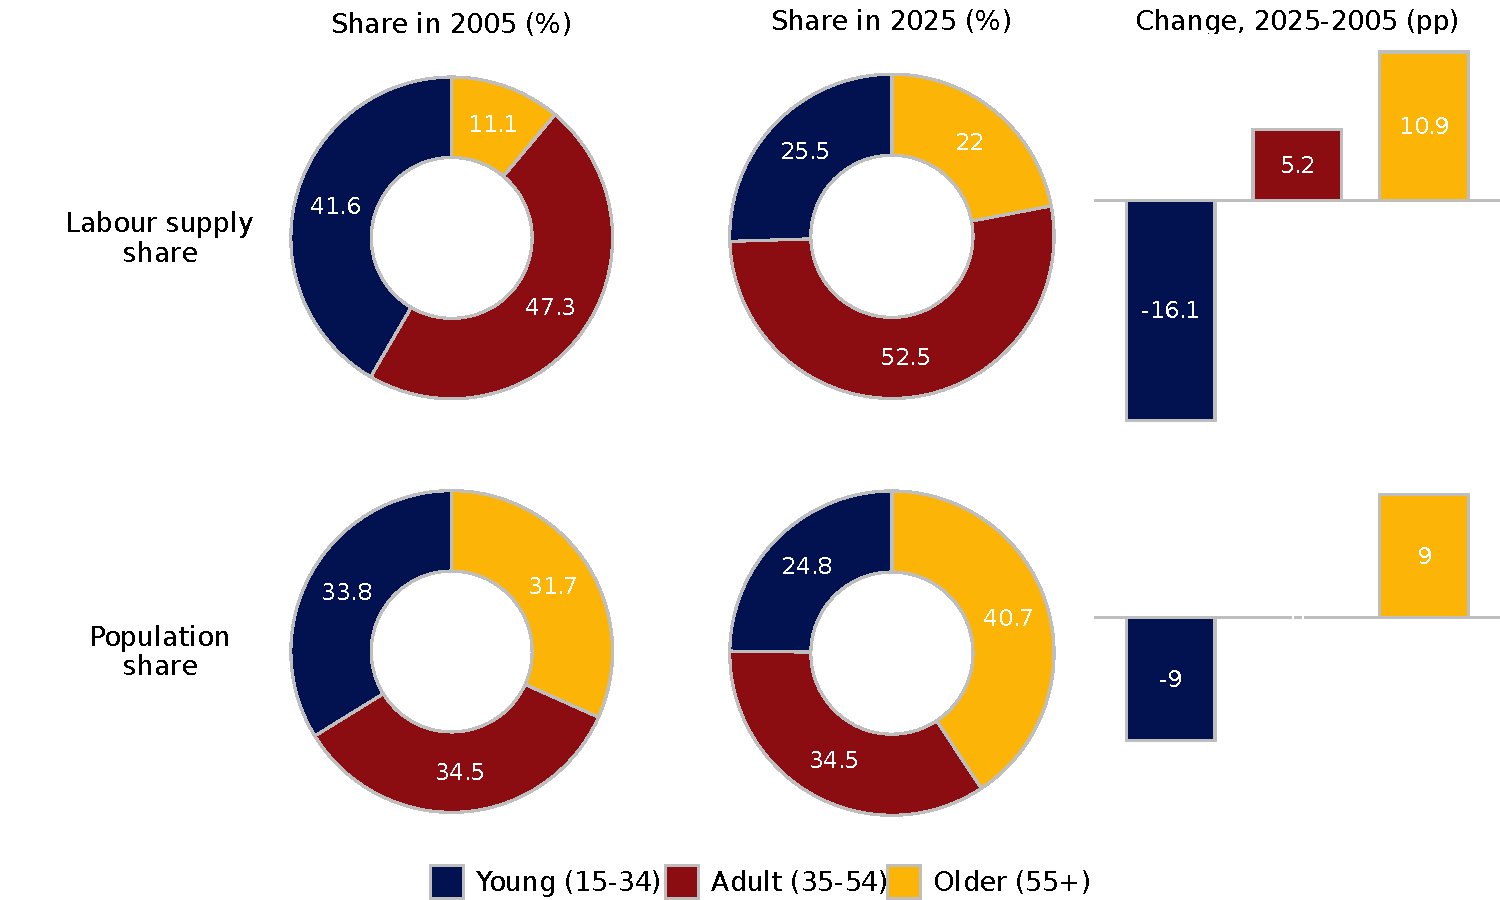
\includegraphics[width=1\textwidth]{../resrc/labPopChg.pdf}%
  \label{fig:labPopChg}%
\end{figure}%


Between 2005 and 2025, Spain’s labour supply shifted strongly away from young workers and toward older and prime-age workers. The young group, aged 15-34, declined from 41.6\% to 25.5\% of aggregate labour supply, a fall of 16.1 percentage points. This drop is much larger than their population-share decline of 9.0 percentage points, suggesting that demographic change alone does not explain the fall. Older workers, aged 55+, moved in the opposite direction. Their population share increased by 9.0 percentage points, from 31.7\% to 40.7\%, but their labour-supply share increased even more, from 11.1\% to 22.0\%, a rise of 10.9 percentage points. This implies that older individuals are contributing more to labour supply not only because they are more numerous, but also because they are more attached to the labour market than before. This behavioral change regarding labour attachment is even more prevalent among the prime-age adults whose contribution to the employment has increased by 5pp despite no change in their population share. In short, Spain’s ageing population does not mechanically reduce aggregate labour supply. The figure shows that behavioural changes, especially higher labour-market contribution among older and prime-age adults, partly offset demographic ageing, while the sharp decline among young workers reflects both demographic shrinkage and weaker labour-supply attachment. And to this, immigration has played a decisive role, as the next figure will show.



\subsection{Labour-Supply Growth by Age and Birthplace}

\begin{figure}[H]%
  \caption{Trend of the aggregate labor supply as a percentage of its level at the beginning of the period, by age group for spanish and immigrants, Spain 2005-2025}
  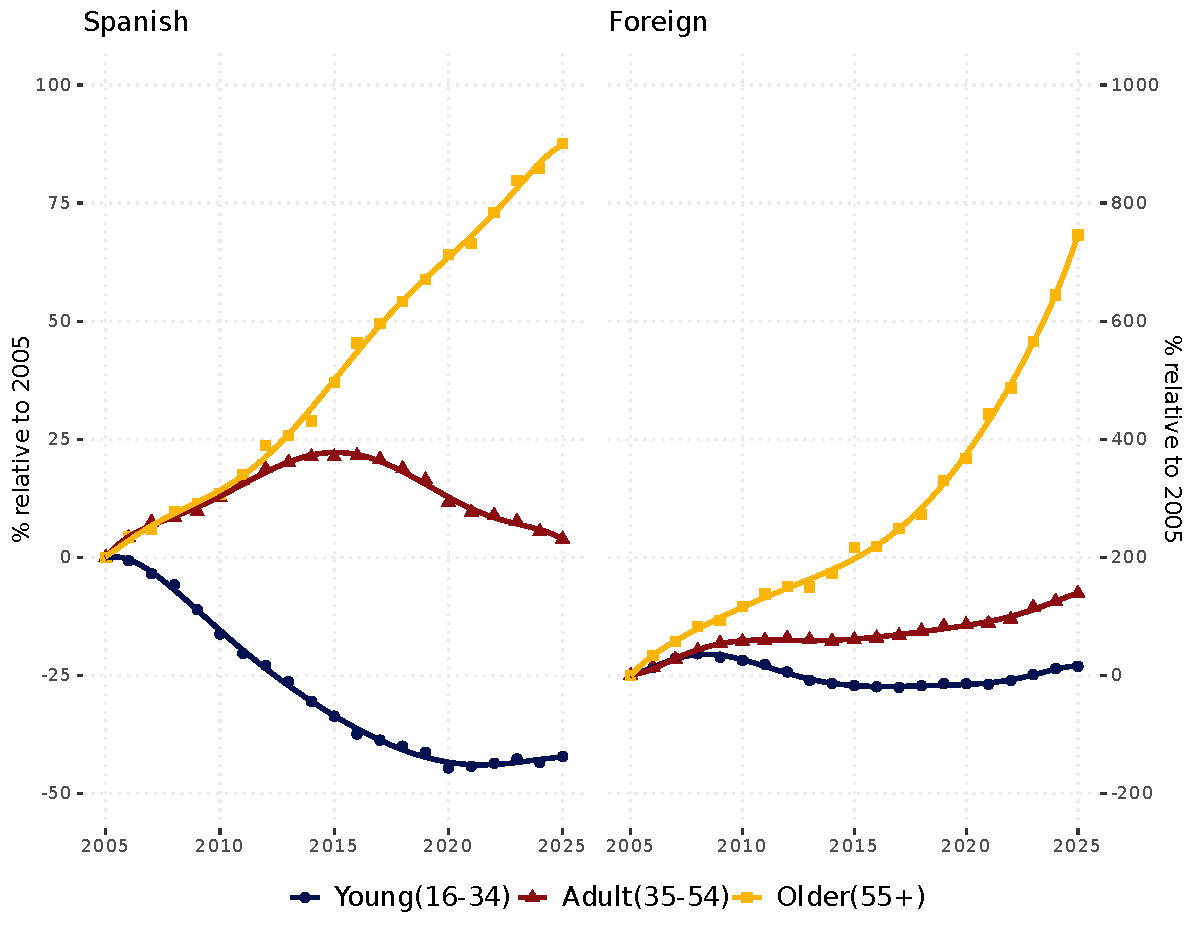
\includegraphics[width=1\textwidth]{../resrc/labRate.pdf}%
  \label{fig:labRate}%
\end{figure}%


The figure shows that immigration is the main source of labour-supply growth, especially among older and prime-age workers. For Spanish, young workers aged 15-34 show a persistent decline in labour supply, falling about 42.2\% below their 2005 level by 2025. Prime-age Spanish aged 35-54 increased until the mid-2010s but returned close to the 2005 level by 2025, only 3.9\% higher. The only strong sustained increase among Spanish is for older workers aged 55+, whose labour supply rose by 87.6\%. For foreigners, the pattern is much more expansionary. Foreign prime-age labour supply increased by 138.9\% relative to 2005, and foreign older labour supply rose by 745.9\%. Young foreign workers are more volatile: they rose before the financial crisis, declined after 2008, and recovered to 15.5\% above the 2005 level by 2025. In short, the figure suggests that Spain’s aggregate labour-supply adjustment is not driven only by ageing among natives. Immigration plays a decisive role by expanding the labour contribution of foreign adults and, especially, older foreign workers, while young native labour supply continues to contract.














\section{Decomposition of Labour-Supply Change}

\subsection{The model of continuous change: an overview}

To measure the isolated effect of demographic ageing on aggregate labour supply, this article uses the continuous-change model \citep{horiuchiDecompositionMethodBased2008}. This model decomposes the difference between two summary measures generated by the same process into several components, each representing the contribution of an underlying factor. The process is defined as a function \(f\), which takes the values of the factors as arguments and returns a summary measure. A technical summary of the method is provided in the annex.

\vspace{0.7em}\par
For each pair of consecutive years between 2005 and 2025, the decomposition allocates the change in aggregate labour supply using a nested three-level structure. The first level separates contributions by birthplace status, distinguishing Spanish and foreign-born populations. Within each birthplace group, the contribution is divided into four components: total population growth (\textit{tpop}), age structure (\textit{stx}), labour-market participation or activity rates (\textit{wpx}), and hours worked (\textit{whx}). Finally, within each component, the contribution is split across age groups. Each contribution piece therefore represents the change in labour hours attributable to a specific age group within a specific component and birthplace group.


\vspace{0.7em}\par
A potential concern with the continuous-change model (CCM) is that it assumes smooth transitions between states, whereas Spain’s labour market was marked by sharp regime changes during the Great Recession, the migration reversal after 2008, and the COVID--19 shock. Although these episodes clearly violate economic smoothness, the CCM remains appropriate for the present analysis for two main reasons.

\vspace{0.7em}\par
First, the CCM does not impose continuity in economic outcomes or behavioural adjustments; continuity applies only to the accounting path used to allocate observed changes across factors. Abrupt movements in employment, migration, or participation are therefore fully captured in the underlying data, and the decomposition integrates these discrete changes mechanically over time without smoothing or averaging away shocks. Moreover, the decomposition is implemented on a year-by-year basis and reported over sub-periods that closely correspond to major regime shifts (2005--2009, 2010--2014, 2015--2019, and 2020--2025). This effectively yields a piecewise application of the CCM, allowing crisis-period dynamics to be identified explicitly rather than diluted within longer trends.

\vspace{0.7em}\par
Second, a central property of the CCM is its additivity, which holds by construction even in the presence of structural breaks. As illustrated in Table \ref{tab:effectMat}: the sum of the contribution pieces across all consecutive-year decompositions equals the corresponding contribution obtained from a decomposition between the first and last years. In addition, the sum of all contribution pieces equals the observed difference in aggregate labour supply between the two years, before decomposition. During crisis periods, this additivity should be interpreted strictly as an accounting identity rather than as evidence of economically smooth adjustment mechanisms. The CCM is thus used as a descriptive tool to allocate observed changes in labour supply across demographic and behavioural components, not as a model of adjustment dynamics.

\vspace{0.7em}\par
Taken together, these features make the CCM a transparent and internally consistent framework for assessing how ageing, migration, participation, and hours worked contribute to labour-supply change, even in periods marked by pronounced labour-market disruptions.






\subsection{Demographic and Behavioural Contributions}

Table \ref{tab:effectMat} shows the contribution of each component by birthplace and period, expressed in millions of full-time equivalent (FTE) workers, where one FTE corresponds to 2,000 annual hours worked. Positive values indicate contributions that increase aggregate labour supply; negative values indicate contributions that reduce it. The table shows that Spain's aggregate labour supply increased by \(2.18\) million FTE workers between 2005 and 2025, but this net gain hides a strong contrast by birthplace. The foreign-born contribution was strongly positive, adding \(3.04\) million FTE workers, while the Spanish contribution was negative, reducing labour supply by \(0.86\) million FTE workers.


\begin{table}[H]%
  \caption{Decomposition of changes in aggregate labour supply by birthplace, component, and period, Spain.}

  %\source{Author's calculations}
  \label{tab:effectMat}%
  \begin{center}
    \input{../resrc/effectMat.tex}%
    \caption*{\small Note: Values are expressed in millions of full-time equivalent (FTE) workers.}
  \end{center}
\end{table}%



\vspace{0.7em}\par
The main negative force is age structure among Spanish. For Spanish, the age-structure component reduced labour supply by \(2.55\) million FTE workers over 2005--2025. This confirms that population ageing among Spanish exerted a large downward pressure. However, this was more than offset by higher Spanish activity rates, which added \(2.82\) million FTE workers, while Spanish population size added \(0.46\) million. Declining hours worked reduced Spanish labour supply by another \(1.60\) million. For foreigners, the main positive contribution comes from population size, which added \(3.56\) million FTE workers. By contrast, foreign age structure slightly reduced labour supply by \(0.14\) million, foreign activity rates contributed almost nothing over the full period, at \(0.01\) million, and foreign hours worked reduced labour supply by \(0.39\) million. This means immigration's contribution came mainly through foreign population growth, not through higher participation or longer hours.

\vspace{0.7em}\par
Across periods, the strongest positive aggregate change occurred in 2005--2009, at \(1.64\) million FTE workers, and 2020--2025, at \(1.17\) million FTE workers. The period 2010--2014 was negative, at \(-0.57\) million, reflecting crisis-era weakness, while 2015--2019 was also slightly negative, at \(-0.05\) million. Overall, foreign population growth offset much of the negative age-structure effect among Spanish, but declining hours worked remained a drag across both groups. The relative contribution of these components across the major age groups is summarized in Figure \ref{fig:labDecomp}.


\subsection{Contribution of Ageing and Labour Components}

Figure \ref{fig:labDecomp} contains three panels distinguishing Spanish, foreign-born, and combined contributions to total labour-supply change between 2005 and 2025. Within each panel, the four bars correspond to the decomposition components: total population growth (\textit{tpop}), age structure (\textit{stx}), activity or participation rates (\textit{wpx}), and hours worked (\textit{whx}). The age-group contribution pieces are grouped into three major age groups: young workers aged 16--34, adults aged 35--54, and older workers aged 55 and over. These age-group contributions are divided by the total change in aggregate labour supply, so each bar represents the percentage of total change attributable to a specific age group within a specific component and birthplace group. For the Spanish and foreign panels, the age-group contributions across all components sum jointly to 100\%, because these two panels add up to the total change in aggregate labour supply. In contrast, the combined panel aggregates Spanish and foreign contributions first; within this panel, the age-group contributions across all components also sum to 100\%. Positive values indicate contribution pieces that increased labour supply, while negative values indicate contribution pieces that reduced it.

\begin{figure}[H]%
  \caption{Contribution of demographic and behavioural factors expressed as a percentage of the total variation in aggregate labour supply, Spain 2005--2025}%
  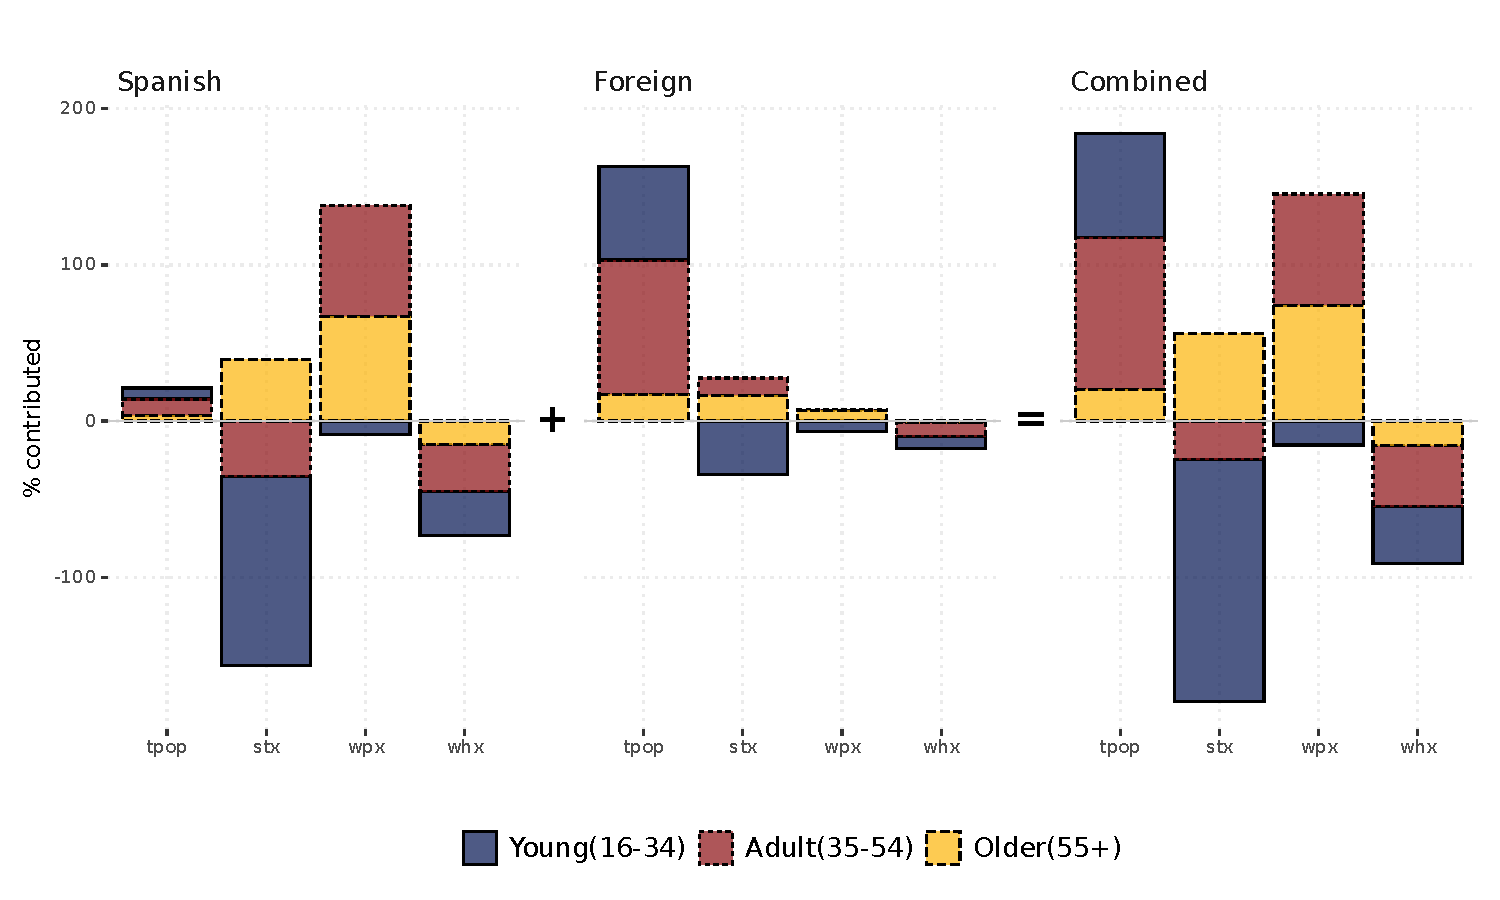
\includegraphics[width=1\textwidth]{../resrc/labDecomp.pdf}%
  \label{fig:labDecomp}%
\end{figure}%




By far, the largest negative contributions come from age-structure changes among younger and prime-age groups. The strongest drag is the age-structure effect for young Spanish aged 16--34, which contributes \(-120.8\%\) of the total change, followed by the age-structure effect for Spanish adults aged 35--54, at \(-35.6\%\). The age-structure effect for young foreigners is also negative, at \(-34.2\%\). In contrast, the largest positive contributions come from foreign population growth among adults aged 35--54, which contributes \(86.3\%\), and from higher activity rates among Spanish adults and older workers, contributing \(70.9\%\) and \(67.1\%\), respectively. Thus, the main offset to demographic ageing within the Spanish-born population comes from foreign prime-age population growth and stronger labour-market attachment among Spanish adults and older workers.





\section{Implication discussion}

The results show that immigration has played a decisive role in offsetting the labour-supply losses associated with population ageing, but they also point to the limits of relying on immigration alone. Ageing affects labour supply not only through population structure, but also through behavioural responses, health, hours worked, and exposure to labour-market shocks. The following subsections therefore discuss three implications of the results: the extent to which immigration compensates for ageing, the potential role of healthy ageing as a complementary strategy, and the risks created by future economic and technological disruptions.


\subsection{Compensating for ageing and the volatility trap}


The age-structure effect among Spanish reduced aggregate labour supply by \(2.55\) million FTE workers over 2005--2025. Immigration more than compensated for this loss: the total foreign-born contribution added \(3.04\) million FTE workers, equal to about \(119.4\%\) of the negative Spanish age-structure effect. In short, without immigration, Spanish ageing would have reduced labour supply substantially; with immigration, the aggregate effect becomes positive. Howerver, this migratory buffer exhibits significant pro-cyclical volatility. As evidenced in the 2010--2014 sub-period (Table 3), the foreign-born contribution turned sharply negative (\(-0.54\) million FTE). This reveals a ``volatility trap'': the primary mechanism for offsetting long-term ageing tends to stall or reverse precisely when the economy faces structural stress \parencite{galvez2022cyclicality, funcas2024vulnerability}.

\vspace{0.7em}\par
The role of immigration should also be assessed in light of alternative adjustment mechanisms, especially the behavioural changes induced by ageing. Contrary to migratory buffers, behavioural adjustments among the Spanish-born population proved more resilient to economic cycles. Higher activity rates added \(2.82\) million FTE workers, which, despite a reduction of \(1.60\) million due to declining hours, resulted in a net positive behavioural contribution of \(1.23\) million FTE. Thus, behavioural adjustment helped offset about \(48.1\%\) of the negative age-structure effect among Spanish. While immigration remains the dominant quantitative offset, its reliability as a stabilizer is contingent on economic growth. This highlights that the requirement for migration to balance ageing could be lowered if policy shifted toward supporting the more stable margin of healthy ageing, potentially decoupling labour supply from the boom-bust cycles of migratory flows \parencite{cepr2025limits}.


\subsection{Investment in healthy ageing as a structural stabilizer}

The importance of healthy ageing as a stabilizer is underscored by recent cross-country evidence. Using data for populations aged 50+ in 41 countries from 2000--2022, \textcite{gruss2025healthyAging} find that a decade of cognitive health gains raises labour-force participation by about 20 percentage points, weekly hours worked by around 6 hours, labour productivity by roughly 30\%, and annual labour earnings by about 35\%. In the Spanish context, such investments are increasingly critical not just for the native population, but for a foreign-born population that is ageing more rapidly than in previous decades.

\vspace{0.7em}\par
The transition from the ``exceptional'' migratory wave of the early 2000s \parencite{arango2013exceptional} to a more settled demographic has altered the foreign-born contribution profile in the 2020s \parencite{bde2023ageingParticipation,caixabank2017labourForceAgeing}. Between 2005 and 2025, the share of foreigners aged 55+ increased from \(11.01\%\) to \(23.85\%\), a rise of \(12.84\) percentage points. This demographic maturation has led to a decline in labour-market intensity: the foreign activity rate fell by \(3.33\) percentage points (from \(74.77\%\) to \(71.44\%\)), and average weekly hours dropped by \(2.58\) hours. Without targeted investments in healthy ageing for this settled population, the ``migration buffer'' may become increasingly inefficient, as the volume of new arrivals would need to rise exponentially just to compensate for the declining intensity of the existing, ageing foreign-born stock \parencite{bde2023ageingParticipation, caixabank2017labourForceAgeing}.


\subsection{Disruption on the horizon and the labour supply}

Immigrants are not only ageing more rapidly than the Spanish-born population, but they are also more exposed to labour-market volatility. Foreign workers were disproportionately affected by the 2008 financial crisis: immigrant employment declined, immigration inflows fell by more than 50\% between 2008 and 2013, and Spain experienced net migration outflows \parencite{rodriguez2016labor}. During COVID-19, the unemployment gap between foreign-born and native workers increased from 6.7 to 10 percentage points by late 2020 \parencite{centaur2021,fasani2023,lacaixa2021}. These facts do not contradict the positive demographic contribution of immigration; rather, they show that immigration is more vulnerable to labour-market disruption. This vulnerability also raises a broader question about how ongoing AI disruption may affect labour-market outcomes for immigrants and for the population more generally. At this stage, the evidence remains fragmented and inconclusive \parencite{pizzinelli2023aiExposure}. Some studies find only small effects, or no clear effect, on labour demand in AI-exposed occupations \parencite{hartley2024labor,Ghosh2025AIExposure}. However, because AI has been shown to raise productivity in several work settings \parencite{DellAcqua2024AIProductivity,Noy2023ProductivityAI}, future increases in output may require fewer additional workers than in the past. If so, Spain may not need to rely on immigration to expand labour supply to the same extent as it did over the last two decades.


\section{Conclusion}

Overall, population ageing substantially reduced Spain's potential labour supply, but behavioural adjustment offset much of this loss. Higher participation, especially among Spanish adults and older workers, helped cushion the demographic shock, although declining hours worked limited the size of this compensation. Immigration filled the remaining gap by expanding labour supply mainly through population growth and age composition. However, this contribution depends on migrants' labour-market integration, sectoral exposure, and employment stability \parencite{preston2014effect,fiorio2023migration,naumann2021population}, making it vulnerable to economic and technological disruptions. For the coming decades, complementary strategies may therefore be needed. In particular, investment in healthy ageing appears promising because it can support longer working lives and strengthen labour‑market attachment among older workers in both the Spanish‑born and foreign‑born populations.

\section{Annexes}

\subsection{Decomposition by continuous change}

The model of continuous change \citep{horiuchiDecompositionMethodBased2008} is used to decompose the change in aggregate labour supply between 2005 and 2025 (the dependent summary measure) into additive effects associated with changes in demographic and behavioural components (the covariates). The model decomposes the difference between two summary measures generated by the same process into several components, each representing the contribution of an underlying factor. The process is defined as a function \(f\), which takes the values of the factors as arguments and returns a summary measure.

\vspace{0.7em}\par
\citet{horiuchiDecompositionMethodBased2008} demonstrates that as the factors transition from values \(x_i(t_1)\) to \(x_i(t_2)\) between two times \(t_1\) and \(t_2\), the summary measure changes from \(f(x_i(t_1))\) to \(f(x_i(t_2))\), and the difference between these two measures can be decomposed into additive components \(c_{i}\) representing the contribution of changes within each factor to this difference. This is expressed by equation \eqref{eq:hofr}.

\begin{equation} \label{eq:hofr}
    f(x_i(t_2)) - f(x_i(t_1)) = \displaystyle\sum_{i}c_{i}
\end{equation}

\vspace{0.7em}\par
With \(i = 1, 2, ..., n\) being the factors involved. The decomposition is based on the assumption that the change in the covariate \(x_i\) occurs continuously or gradually over a real or hypothetical time dimension \(t_1 \rightarrow t_2\). This provides a reasonable justification for the additivity of the effects of the factors and the elimination of interaction terms even if the process in question is a non-additive function of the covariates \citep[p.~786]{horiuchiDecompositionMethodBased2008}.

\vspace{0.7em}\par
In other words, the continuous change model (CCM) introduces a decomposition function \(g\) which, using a process function \(f\), transforms two series of covariates, the vectors \(X(t_1)\) and \(X(t_2)\) representing the values of the covariates \(X = (x_1, ..., x_i, ..., x_n)\) at times \(t_1\) and \(t_2\), into a series of contributions or effects, the vector \(C = (c_1, ..., c_i, ..., c_n)\). Thus, we can write:

\begin{equation}\label{eq:gfr}
    C = g(X, f)
\end{equation}

The series \(X\) and \(C\) having the same lengths, results in a perfect correspondence between the factors and the effects, which can be grouped for analysis purposes. Furthermore, the idea of continuity implies that each element \(c_i\) of the series \(C\) is obtained by integration according to the equation:

\begin{equation}\label{eq:mxfr}
    c_i = \int_{x_i(t_1)}^{x_i(t_2)} \frac{\partial f(t)}{\partial x_i(t)} dx_i(t)
\end{equation}

In practice, equation \eqref{eq:mxfr} is estimated by numerical integration where \(\int_{x_i(t_1)}^{x_i(t_2)} d(t)\) is approximated by \(\sum_{x_i(t_1)}^{x_i(t_2)} \delta(t)\), with \(x_{it} = x_i(t)\) being the value of a factor \(i\) at a moment \(t\). Adapting the continuous change model to measure equation \eqref{eq:pclab} allowed the total variation in the aggregate labor supply between 1981 and 2016 to be distributed not only among these three components but also by age group and residence status (immigrants and natives). For this article, the decomposition was performed by creating an auxiliary function \(g\) around the R package \citep{Rstat:2018} DemoDecomp \citep{DemoDecomp:2018}. The code and data used are available upon request.

\vspace{0.7em}\par
The CCM model is a better alternative to the standardization method often used in demography to account for differences in population structure when comparing demographic measures. Indeed, standardization requires a third population to serve as a standard, making it somewhat less robust as different standards can lead to different results. The CCM model solves this problem and allows for direct decomposition without interaction terms between the different factors.

Interaction effects in regression analysis refer to situations where the impact of one variable on a dependent variable is not constant or additive but depends on the values of other variables. In traditional decomposition methods, such as standardization, any discrepancy between the overall change and the sum of the individual effects of the variables is also called an interaction effect. In such cases, the interaction represents an incomplete separation of the contributions of individual covariates to the overall change or difference in a dependent variable.


\subsection*{Data Source and Variables}

The analysis uses microdata from the \textit{Encuesta de Población Activa} (EPA), Spain's quarterly Labour Force Survey produced by the National Statistics Institute (INE). The EPA is a nationally representative household survey covering the population aged 16 and over. It follows a stratified, two-stage sampling design, with census sections as primary sampling units and dwellings as secondary units. Each quarterly wave includes approximately 46{,}000 dwellings and more than 100{,}000 individuals. INE provides calibrated survey weights to ensure consistency with population totals by sex, age, and region. The microdata contain detailed demographic characteristics, labour-force status, employment conditions, hours worked, and place of birth. The original variables used from the microdata files are:

\begin{itemize}
    \item \textbf{FACTOREL (survey weight)}: Expansion factor assigned to each respondent, derived from the sampling design and calibrated to external population benchmarks. It is used to compute weighted totals and representative aggregates.

    \item \textbf{EDAD1 / EDAD5 (age group)}: Age information is provided in grouped intervals. Across releases, the relevant age-group variable appears as either \textit{EDAD1} or \textit{EDAD5}, but both use five-year age groups for the analytical period. The analysis uses whichever variable is available and standardises it into a single age-group variable.

    \item \textbf{AOI (labour-force status)}: Constructed by INE from responses on work activity, job search, and availability. \textit{AOI} classifies individuals as employed, unemployed, or inactive. It is used to identify employed persons and the active population.

    \item \textbf{HORASH (effective weekly hours worked)}: For employed respondents, the EPA records actual hours worked in the reference week, including overtime and excluding absences. These responses are coded into \textit{HORASH} and used to compute average hours and total hours supplied.

    \item \textbf{PRONA1 (province or country of birth)}: Respondents report their place of birth, which INE codes as Spanish provinces or foreign countries. This variable is used to distinguish Spanish-born from foreign-born individuals.
\end{itemize}


\subsection{Trend in labour force components}

\begin{figure}[H]%
    \caption{Average participation rate by major age groups for immigrants and natives, Spain 2005-2025}
    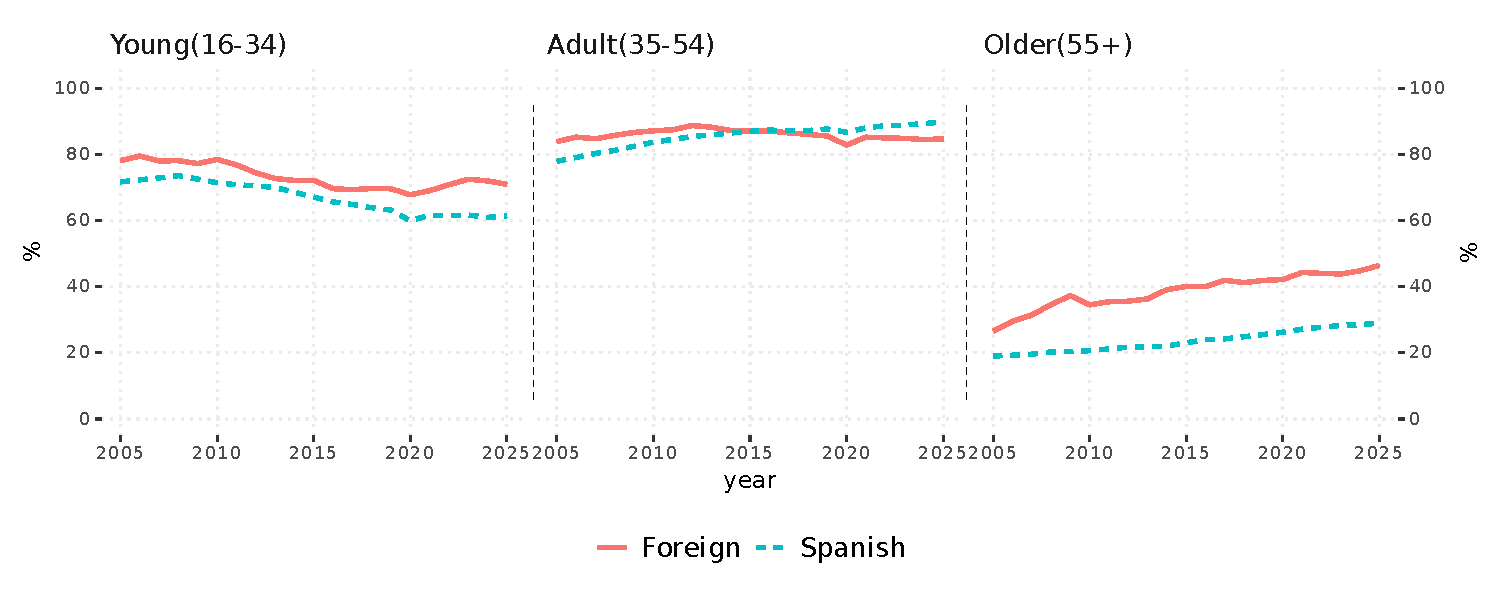
\includegraphics[width=1\textwidth]{../resrc/wpx.pdf}%
    \label{fig:wpx}%
\end{figure}%

\begin{figure}[H]%
    \caption{Average worked hours by major age groups for immigrants and natives, Spain 2005-2025}
    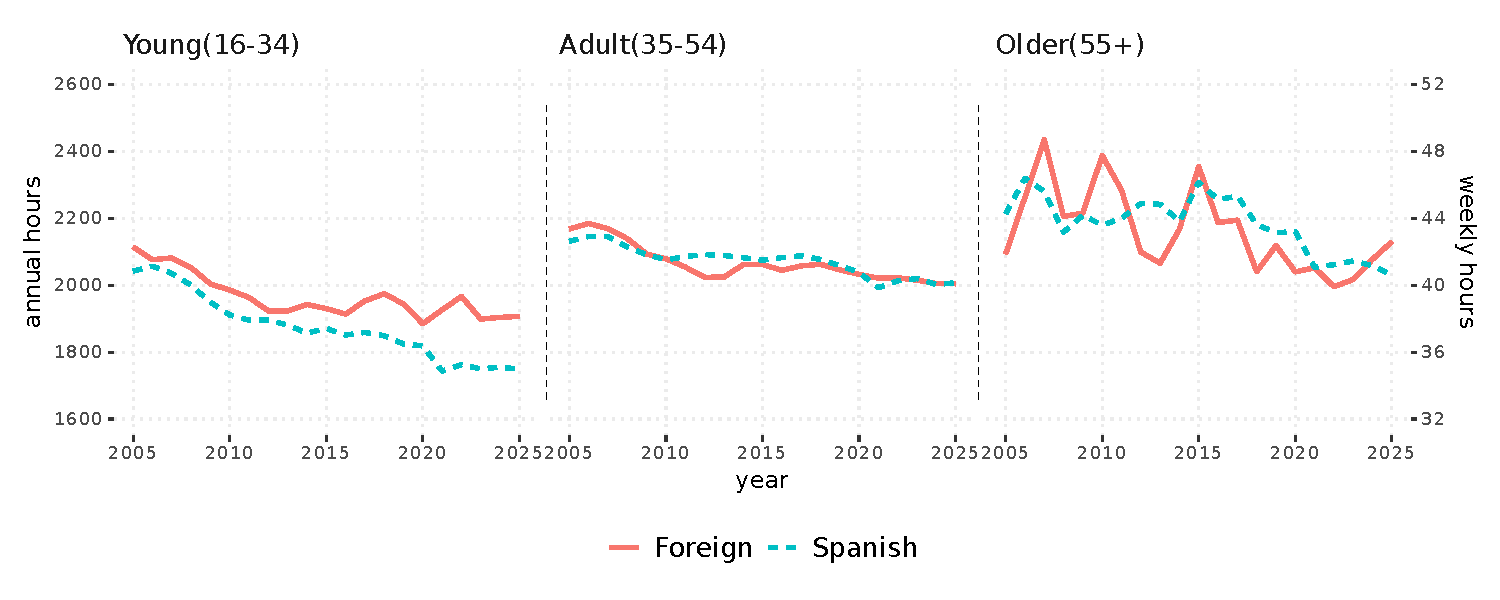
\includegraphics[width=1\textwidth]{../resrc/whx.pdf}%
    \label{fig:whx}%
\end{figure}%

\begin{figure}[H]%
    \caption{Percentage of total population by major age groups for immigrants and natives, Spain 2005-2025}
    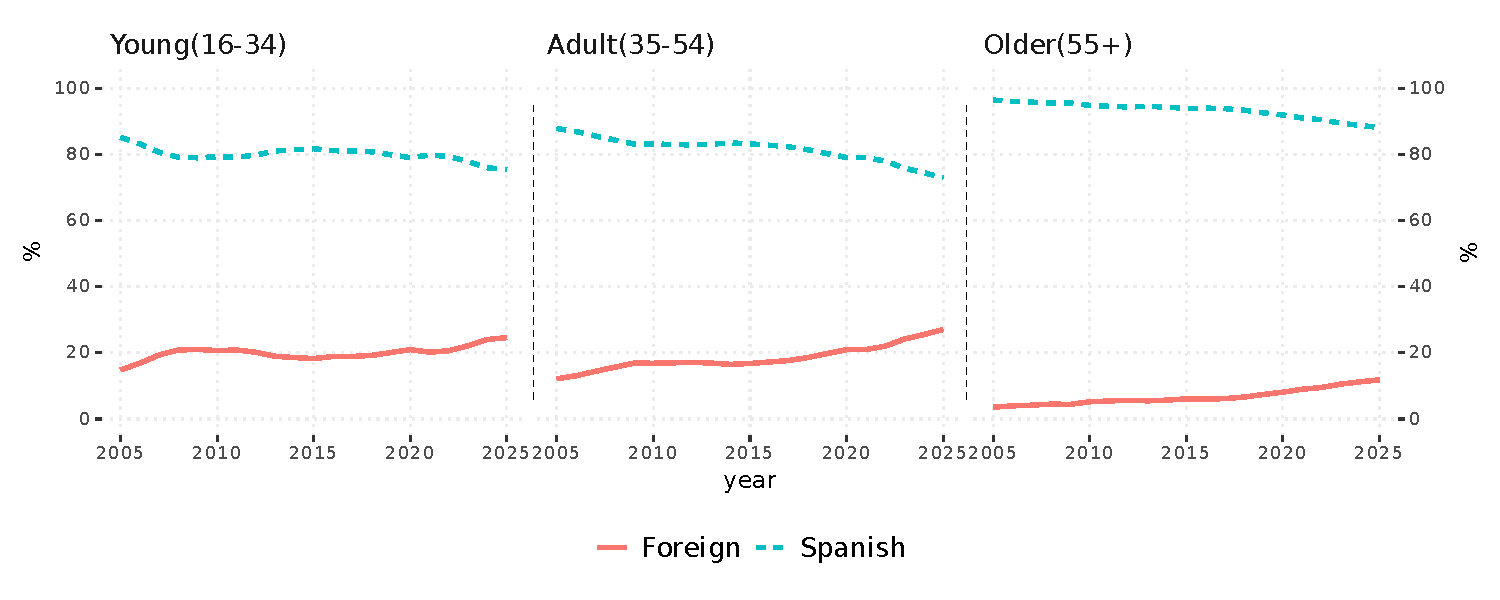
\includegraphics[width=1\textwidth]{../resrc/stx.pdf}%
    \label{fig:stx}%
\end{figure}%

\begin{figure}[H]%
    \caption{Total population aged 16+ in full-time equivalent (FTE) by birthplace, Spain 2005-2025}
    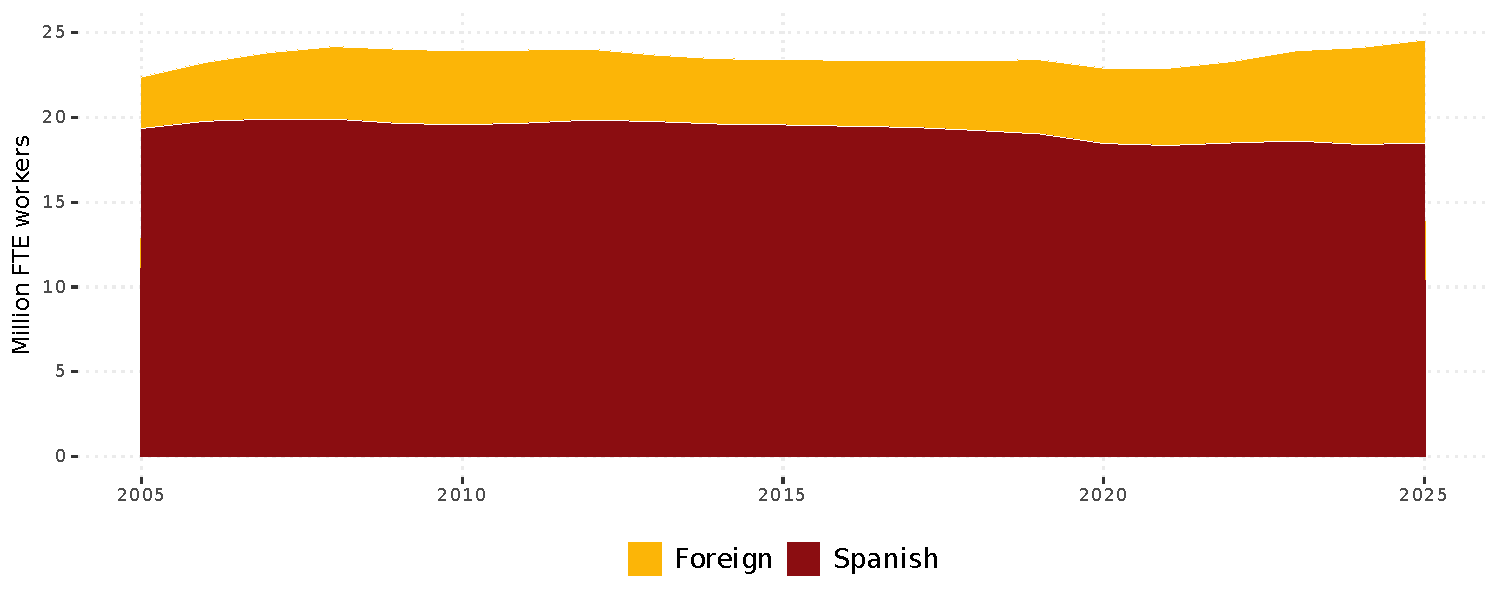
\includegraphics[width=1\textwidth]{../resrc/labchg.pdf}%
    \label{fig:labchg}%
\end{figure}%


% reference
\section*{References}
%\addcontentsline{toc}{section}{References}
\printbibliography[heading=none]

\end{document}
